\begin{problem}
Плотность распределения СВ \(\xi\) имеет вид:
\[
    f_\xi(x) = \begin{cases}
        c(1 - x^2), & |x| \leqslant 1 \\
        0,          & | x | > 1
    \end{cases}
\]
Найти:
\begin{enumerate}[label=\alph*)]
    \item константу c
    \item функцию распределения СВ \(\xi\)
    \item построить график функции плотности распределения СВ и график функции распределения СВ
    \item \(\mathbb{E}(2 - \xi)(4 + 3\xi)\)
    \item \(\mathbb{D}(5 - 2\xi)\)
    \item \(\mathbb{P}(\xi > 0.5)\)
\end{enumerate}
\end{problem}

\begin{solution} \
    \begin{enumerate}[label=\alph*)]
        \item Найдем константу из условия нормировки :
              \[
                  1 = \int_{-\infty}^{\infty} f_\xi(x) dx = \int_{-1}^1 c(1 - x^2) dx = c\left(x - \frac{x^3}{3}\right)\bigg{|}_{-1}^1 = c \left( 1 - \frac{1}{3} \right) - c\left(-1 + \frac{1}{3}\right) = c \cdot \frac{4}{3}
              \]
              \[
                  \Downarrow
              \]
              \[
                  c = \frac{3}{4}
              \]

        \item \(F_\xi(x) = \int_{-\infty}^x f_\xi(t) dt = \begin{cases}
                  1,                                   & x > 1            \\
                  \int_{-1}^x \frac{3}{4}(1 - t^2) dt, & -1 \leqslant x \leqslant 1 \\
                  0,                                   & x < -1
              \end{cases}\) \\\\
              Отдельно:
              \[
                  \int_{-1}^x \frac{3}{4}(1 - t^2) dt = \frac{3}{4} \left( t - \frac{t^3}{3} \right) \bigg|_{-1}^x = \frac{3}{4} \left( x - \frac{x^3}{3} \right) - \frac{3}{4} \left( -1 + \frac{1}{3} \right) = \frac{3}{4} \left( x - \frac{x^3}{3} \right) + \frac{1}{2}
              \]
              Тогда функция распределения:
              \[
                  F_\xi(x) = \begin{cases}
                      1,                                                          & x > 1            \\
                      \frac{3}{4} \left( x - \frac{x^3}{3} \right) + \frac{1}{2}, & -1 \leqslant x \leqslant 1 \\
                      0,                                                          & x < -1
                  \end{cases}
              \]
        \item \[
                  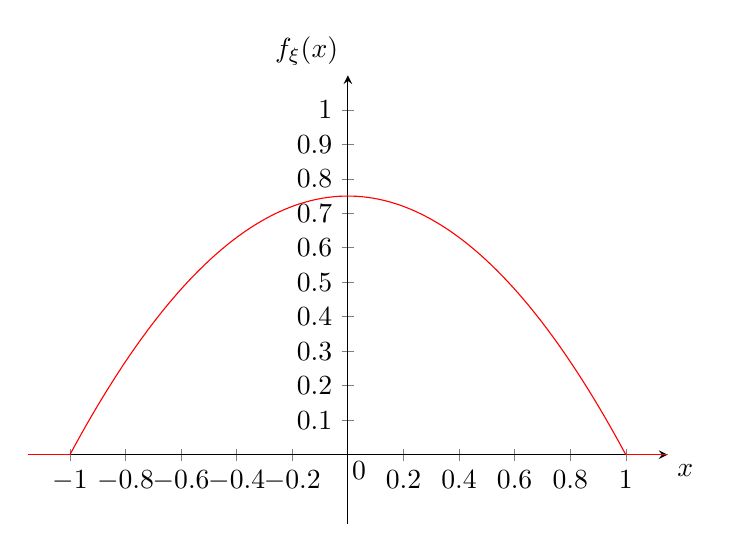
\begin{tikzpicture}[>=latex]
                      \begin{axis}[
                              width=0.8\textwidth,
                              height=0.6\textwidth,
                              axis x line=center,
                              axis y line=center,
                              xtick={-1.4,-1.2,...,1.4},
                              ytick={0,0.1,...,1},
                              xlabel={$x$},
                              ylabel={$f_\xi(x)$},
                              xlabel style={below right},
                              ylabel style={above left},
                              xmin=-1.15,
                              xmax=1.15,
                              ymin=-0.2,
                              ymax=1.1,
                              legend style={nodes={scale=1}}]

                          \addplot [domain=-1:1,color=red, samples=100] {3/4*(1-x*x)};
                          \addplot [domain=-1.5:-1,color=red, samples=100] {0};
                          \addplot [domain=1:1.5,color=red, samples=100] {0};
                          \node at (axis cs:0.04,-0.045) {$0$};
                      \end{axis}
                  \end{tikzpicture}
              \]

              \[
                  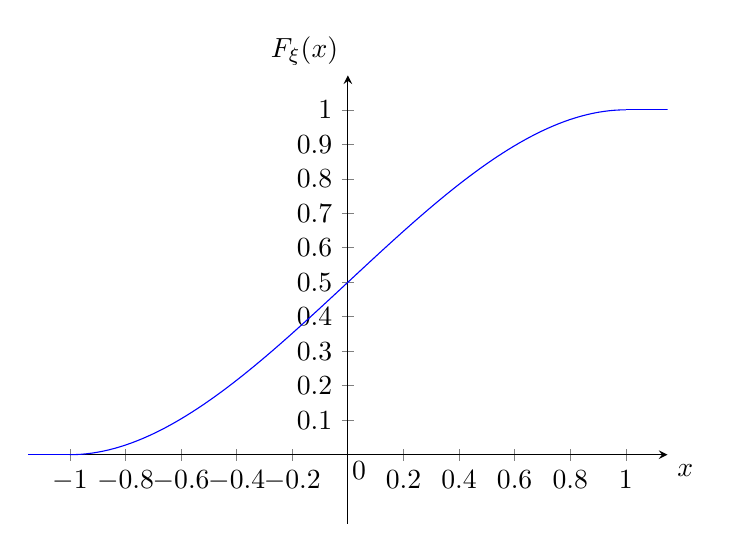
\begin{tikzpicture}[>=latex]
                      \begin{axis}[
                              width=0.8\textwidth,
                              height=0.6\textwidth,
                              axis x line=center,
                              axis y line=center,
                              xtick={-1.4,-1.2,...,1.4},
                              ytick={0,0.1,...,1},
                              xlabel={$x$},
                              ylabel={$F_\xi(x)$},
                              xlabel style={below right},
                              ylabel style={above left},
                              xmin=-1.15,
                              xmax=1.15,
                              ymin=-0.2,
                              ymax=1.1,
                              legend style={nodes={scale=1}}]

                          \addplot [domain=-1:1,color=blue, samples=100] {3/4*(x - x*x*x/3) + 1/2};
                          \addplot [domain=-1.5:-1,color=blue, samples=100] {0};
                          \addplot [domain=1:1.5,color=blue, samples=100] {1};
                          \node at (axis cs:0.04,-0.045) {$0$};
                      \end{axis}
                  \end{tikzpicture}
              \]

        \item \[
                  \mathbb{E}(2 - \xi)(4 + 3\xi) = \mathbb{E}(8 + 2 \xi - 3\xi^2) = 8 + 2 \mathbb{E}\xi - 3 \mathbb{E}\xi^2
              \]
              Найдем отдельно \(\mathbb{E}(\xi)\):
              \[
                  \mathbb{E}\xi = \int_{-\infty}^{\infty} x f_\xi(x) dx = \int_{-1}^1 x \cdot \frac{3}{4} (1 - x^2) dx = \frac{3}{4} \left( \frac{x^2}{2} - \frac{x^4}{4} \right) \bigg|_{-1}^1 = 0
              \]
              Найдем отдельно \(\mathbb{E}(\xi^2)\):
              \[
                  \mathbb{E}\xi^2 = \int_{-\infty}^{\infty} x^2 f_\xi(x) dx = \int_{-1}^1 x^2 \cdot \frac{3}{4} (1 - x^2) dx = \frac{3}{4} \left( \frac{x^3}{3} - \frac{x^5}{5} \right) \bigg|_{-1}^1 = \frac{3}{2} \left( \frac{1}{3} - \frac{1}{5} \right) = \frac{3}{2} \cdot \frac{2}{15} = \frac{1}{5}
              \]
              Тогда:
              \[
                  \mathbb{E}(8 + 2 \xi - 3\xi^2) = 8 + 2 \cdot 0 - 3 \cdot \frac{1}{5} = \frac{37}{5}
              \]

        \item \(\mathbb{D}(5 - 2\xi) = \mathbb{D}5 + \mathbb{D}(-2\xi) = 0 + 4\mathbb{D}\xi = 4 \left( \mathbb{E}\xi^2 - \left( \mathbb{E}\xi \right)^2 \right) = 4 \left( \dfrac{1}{5} - 0 \right) = \dfrac{4}{5}\)
        \item \( \mathbb{P} (\xi > 0.5) = 1 - \mathbb{P}(\xi \leqslant 0.5) = 1 - F_\xi(0.5) = 1 - \left( \dfrac{3}{4} \left( 0.5 - \dfrac{0.5^3}{3} \right) + \dfrac{1}{2} \right) = 1 - 0.84375 = 0.15625\)
    \end{enumerate}
\end{solution}